% Created 2023-05-08 Mon 18:21
% Intended LaTeX compiler: pdflatex
\documentclass[presentation]{beamer}
\usepackage[utf8]{inputenc}
\usepackage[T1]{fontenc}
\usepackage{graphicx}
\usepackage{longtable}
\usepackage{wrapfig}
\usepackage{rotating}
\usepackage[normalem]{ulem}
\usepackage{amsmath}
\usepackage{amssymb}
\usepackage{capt-of}
\usepackage{hyperref}
\usepackage{braket}
\usepackage{listings}
\usepackage{bbm}
\setbeameroption{show notes}
\usetheme{Berlin}
\usefonttheme{professionalfonts}
\author{Yusheng Zhao}
\date{2023-05-10}
\title{Physics behind Computation}
\subtitle{Topological protection from decoherence}
\hypersetup{
 pdfauthor={Yusheng Zhao},
 pdftitle={Physics behind Computation},
 pdfkeywords={},
 pdfsubject={AMAT 5600 Final Presentation},
 pdfcreator={Emacs 28.2 (Org mode 9.6.1)}, 
 pdflang={English}}
\begin{document}

\maketitle
\begin{frame}{Outline}
\tableofcontents
\end{frame}


\section{Motivation}
\label{sec:org7a7ca73}
\begin{frame}[label={sec:org2a5cad1}]{What's Quantum Computer}
\begin{itemize}
\item Information encoded on a qubit: \(\ket{\psi} = \alpha \ket{0} + e^{i\theta}
  \beta \ket{1}\)
\item Operations(gates) are unitary (hence reversible)
\item Quantum Computing has advantage over Classical
\end{itemize}
\end{frame}

\note{Note
\begin{itemize}
\item Quantum Computers could solve some problems more efficiently compared to
classical computers. For example, Shor's algorithm is able to factor large
integers \(N\), in \(\mathcal{O}(log(N)^{2}loglog(N)\) time. Meanwhile, the best
known classical algorithm is \(\mathcal{O}(e^{1.9
  log(N)^{1/3}loglog(N)^{2/3}}\).
\end{itemize}}

\begin{frame}[label={sec:org45cc246}]{Noise in Quantum Computer}
\begin{itemize}
\item Noise is the archenemy
\item Noise is from unwanted local perturbation
\end{itemize}
\end{frame}

\begin{frame}[label={sec:org11148c2}]{Solution}
\begin{itemize}
\item Store information \alert{non-locally}
\item ``If a physical system were to have quantum topological (necessarily nonlocal)
degrees of freedom, which were insensitive to local probes, then information
contained in them would be automatically protected against errors caused by
local interactions with the environment.'' - A. Kitaev
\end{itemize}
\end{frame}
\note{Note
\begin{itemize}
\item However, this technology is plagued by noise. Roughly speaking, noise is like
a little daemon who flips the abucus that you use to do calculation. The
source of those noise come from unwanted physical interaction. or even badly
calibrated actions.
\item For the purpose of this talk, we focus on unwanted physical interaciton.
\item This gives us an idea. Since all known physical interactions are local, could
be store our information non-locally to alleviate the effect of noise?
\end{itemize}}

\section{Topological Protection}
\label{sec:org9e028e3}

\begin{frame}[label={sec:org3a047e8}]{Topological Invariant}
\begin{center}
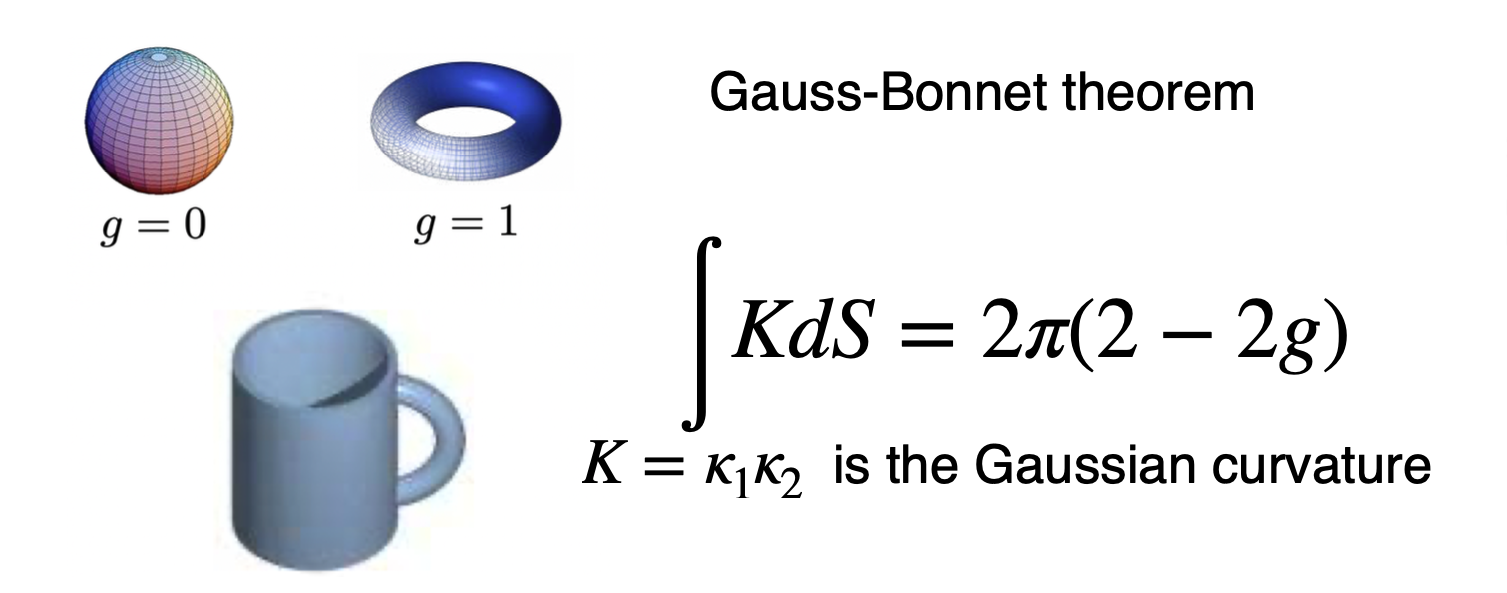
\includegraphics[width=.9\linewidth]{./TopoInvariant.png}
\end{center} [Prof. Li Slides]
\end{frame}

\note{Note
\begin{itemize}
\item Recall our definition of a topological invariant, as previously defined in
class. Both the Gauss-Bonnet theorem and the calculation of the Berry phase
require an integral over the entire system. Local information alone is
insufficient to determine the topological invariants of a system. Similarly,
if one has the ability to alter a system locally, they cannot alter the
topological invariant number of that system.
\end{itemize}}

\begin{frame}[label={sec:org6b31504}]{Topological Degeneracy}
\begin{itemize}
\item Arises from topologically non-trivial phase
\item Protected from local perturbation
\end{itemize}
\end{frame}

\note{Note
\begin{itemize}
\item Using this as a guide, we turn our attention to topological systems. In the
limit of large system size, a topologically non-trivial phase can emerge from
a gapped quantum many-body system. One key feature of the non-trivial phase is
that it possesses topologically degenerate ground states that are not
degenerate in the topologically trivial phase. Therefore, the degeneracy of
the ground states is a direct consequence of the topology of the system's
phase. Applying the logic from the previous paragraph, we expect these ground
states to be protected from local noise, meaning decoherence should not affect
them.
\end{itemize}}

\section{Kitaev's Toy Model}
\label{sec:org5bca09c}
\begin{frame}[label={sec:org87dcd0e}]{Hamiltonian \cite{kitaevUnpairedMajoranaFermions2001}}
\begin{itemize}
\item \(H = \sum_{n=1}^{N} [- \mu (a^{\dagger}_{n}a_{n}- \frac{1}{2}) - w
  (a^{\dagger}_{n}a_{n+1} + a^{\dagger}_{n+1}a_{n}) + \Delta a_{n}a_{n+1} +
  \Delta^{*}a^{\dagger}_{n+1}a^{\dagger}_{n})]\)
\end{itemize}
\end{frame}

\begin{frame}[label={sec:orgc860112}]{Emergence of Non-trivial Phase \cite{huangIntroductionMajoranaZero2021}}
\begin{itemize}
\item \(|\Delta| = w > 0\)
\item \(a_{n} = \frac{1}{2}(e^{-i \theta /2}\gamma_{2n} +
  e^{i\theta/2}\gamma_{2n-1})\), \(\gamma\) is the Majorana creation/anhilation operator
\item \(a^{\dagger}_{n} = \frac{1}{2}(e^{i\theta/2}\gamma_{2n} -
  e^{-i\theta/2}\gamma_{2n-1})\)
\item \(\tilde{a}_{n} = (\gamma_{2n}-i\gamma_{2n+1})/2\)
\item \(H = 2w \sum_{n=1}^{N-1}(\tilde{a}^{\dagger}_{n}\tilde{a}_{n} -1/2)\)
\end{itemize}
\end{frame}

\begin{frame}[label={sec:orgebebd8d}]{A picture is worth a thousand words}
\begin{center}
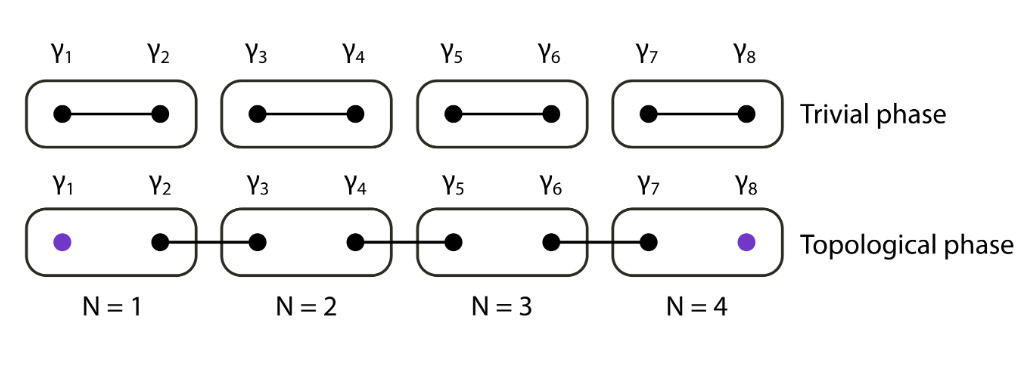
\includegraphics[width=.9\linewidth]{./two-phases.png}
\end{center}
\end{frame}

\note{Note
\begin{itemize}
\item Note, \(\gamma_1\) and \(\gamma_{2N}\) are not in Hamiltonian
\item Have zero energy.
\item Combine to make fermonic mode \(\tilde{a}_{0} =(\gamma_{1}+i\gamma_{2N})/2\)
\item \(\ket{0}\) and \(\ket{1}\) of above creation operator have degenerate energy.
\item Also protected by topology. Can be made into protected qubits!
\end{itemize}}

\section{Take Home Message}
\label{sec:orgdc80415}
\begin{frame}[label={sec:orgb3dc503}]{Physics and Computation}
\begin{itemize}
\item ``Information is Physical'' \cite{landauerThereAreNo1991}
\item Topologically degenerate degree of freedom sees not local perturbation
\end{itemize}
\end{frame}

\note{Note
\begin{itemize}
\item Information is physical, meaning that the effecacy of the computation relies
very much so on the system that realizes it. Computation is not merely
something on the paper. It's very much so related to the physical world.
\item Topological degree of freedom is calculated from the system-wide point of
view. Therefore, it could not be probed locally hence it's immune to local
error.
\end{itemize}}


\section{Bibliography}
\label{sec:org2e54c0a}
\begin{frame}[allowframebreaks]{References}
\bibliographystyle{apalike}
\bibliography{finalp}
\end{frame}
\end{document}